\chapter{Analysis}
\todo{Skrevet om, trengs å leses over}
This chapter provides the background knowledge required to understand the thought process behind the selected technologies.
The Group has been researching different technologies and solutions that can be viable for the application we are developing. Throughout the selection process the group have presented the assignment provider, Michael A. Lundsveen with results from the research and recommendations the group has found for the different technologies that can be used for the application. The group together with Michael worked together to select which technologies that should be used based on the this research.

The chapter first inspects the database technologies that are suitable for the assignment.
Afterwards the chapter examines the selected frontend technology before analyzing the technology stack used for the backend development.
Lastly the chapter provides insight as to why the methodology selected is the most suitable for the project.

\section{Analysis of different MakerSpaces}
The project group has decided to conduct interviews with different MakerSpace branches in Norway. The reason for choosing interviews is to be able to decide what information we want to get out of the interviewees. The project group will make a set of predetermined questions about how MakerSpace operates and what kind of systems and technologies they have. While conducting the interviews the project group also wants to arrange the interview at the respective MakerSpace, where the project group could get a tour of the MakerSpace and take a look at the systems they have and how they are used. This will be used to get more hands-on knowledge for the project, to be able to make a better system. The interviewee will also be more comfortable in a known environment during the interview.

\subsection{MakerSpace Inspiria}

This section is based on an interview the group conducted, as such the necessary sources are added as an attachment. The source is a voice recording of the interview transcribed. \todo{Husk å endre dette}See page::::::::::::: %lage attachement/appendix side for vedlegg?%  

The first MakerSpace that was interviewed was MakerSpace Inspiria, located in Sarpsborg. It is part of Inspiria Science Centre \cite{Inspiria-SC}, a building full of science for people to enjoy and test out. It is mainly targeted for kids, but the MakerSpace is open for everyone when the centre is open. MakerSpace Inspiria is very much alike MakerSpace Halden. It's closely resembles each other and has a lot of the same equipment; 3D printers, laser cutters, soldering irons etc. 
And it is here the group conducted its first interview, at MakerSpace Inspiria. The interviewee answered all the questions best possible and the group got a lot of interesting information. There was no system in place for keeping tabs on the inventory, digital or other. The employees were the ones that kept control over the inventory personally, the employees shared responsibility of overseeing the inventory and ordering new parts and equipment when needed. But admitted to not having full control over everything. Components and tools are being kept in lockers and has a box i.e where similar tools or components are grouped and put together. There is however no special categorizing of the equipment, but everything has a predetermined place. 

As far as lending out equipment, MakerSpace Inspiria has no system in place for it and they do not lend equipment out. Exceptions could be made, depending on the person asking to loan something or the equipment in question. If an exception is made, the employee that loans something out is responsible for the item and its condition. If something is broken or gets broken, MakerSpace Inspiria has a system for reporting broken or faulty equipment. This system is used for the entire building (Inspiria Science Center). The employees report on the specific equipment that is broken and it is filed for review. The review consist of looking at the budget and the broken equipment to see if it is possible to order a replacement or if it is to expensive at the moment. This depends on what kind of equipment is broken. If it is an expensive 3D printer there might not be enough money in the budget to buy a new one e.g However if it is something smaller and not very expensive the employees doesn't report it broken and just orders a new one. 

When asked if a digital system for inventory keeping was something MakerSpace Inspiria could potentially want, the interviewee positively agreed. The interviewee already had an idea for a potential digital system. A simple bar-code and a scanner, zero thinking. Everything has its own ID and it gets scanned into a system. Everything about it has to be simple and have as few button presses as possible. This was from the interviewees own experience with people and IT, or more about people who doesn't know a lot about IT and would be using mentioned system. Other than that the interviewee didn't have any specific ideas on how the system should work or look. But the project group got some very nice ideas and pointers for the User Interface (UI) and User Experience (UX). Keep it nice and simple, not very complicated which is something the project group had already thought of. A bar-code was discussed early on in the project as a possible solution for both lending out equipment and inventory keeping. 

\subsection{Conclusion of the interview and questionnaire}

After an interview and getting 20 questionnaire responses from different MakerSpace's. The group has read through the responses and analyzed them. However, since all the answers are anonymous the group doesn't know which MakerSpace's that responded.   

The equipment each respondent have was varied, everything from digital tools and equipment to more heavy tools like CNC machines, laser cutter, metal saws, vinyl cutters, acids for creating circuit boards and more. Basically every tool for the job to let everyone, children and adults be as creative as possible and give them the space they need for it. 

For any workplace that have tools, it is important to know where everything is. This makes it easier to find what you are looking for. Out of 20 respondents the categorizing and placement of tools went from having no idea or no system, to full control with a website and database for every tool and component. The most common sorting was after the size and type of tool and what department it belonged to (Electronics, Mechanical i.e). Here is a short list of different methods of storing and categorizing tools from MakerSpace's:

\begin{itemize}
    \item "Big things goes in lockers, small things goes on the wall."
    \item "Categorized after which department it belongs to, i.e electronics, metal, wood etc."
    \item "Tools are not categorized and all components counted by stocktaking and saved in a database with potential of resale through own proprietary developed sale system."  
    \item "Every component is sorted after the category i.e transistors, IC, sensors and tools are sorted after usage area and size. There is a designated room for the biggest/baddest/noisiest tools." 
    \item "I have no clue"
    \item "Drawers and shelves etc. On our website you can search i.e for an electronic component and get an overview of what we have and the exact shelf it is located on, but also if the component is available in stock. Sale price is also listed. Heavy machinery like welding gear, wood grinder belongs to a room we call heavy machinery.
    Most of the electronic components are sorted into shelves with a searchable position from our website. However quantity is not always updated, you will need to check yourself if the component you are looking for is available. If we are informed that we have run empty of a component, it will take usually 1-2 weeks before we have bought in more. We sell Arduino, Raspberry pi and touch monitors to customers. We also have two new room where we have a laser cutter and other stuff but the room Isn't fully decorated yet."  
\end{itemize}

Tools, equipment and components can be broken. How the broken item is reported broken and handled afterwards was one of the questions asked. How this is handled with or without a digital system could be important information for how the application is developed and how items in the system should be handled(function as removable by unique id or based on quantity i.e). 
None of the respondents had any digital system for reporting damaged or destroyed tools and components. If anything was broken it was either reported to a superuser or employee by the person that broke or found something broken. Some of the tools and components was considered consumable and just replaced. Certain equipment at one MakerSpace was prohibited from "ordinary users" from using and only certain members was allowed to operate them. Some examples of what equipment was prohibited is; 3D printers, CNC machines, laser cutter and welding tools. The prohibition of the equipment happened after someone broke a very expensive 3D printer. 
Some of the respondents had a form that needed to be filled out and also used Slack internally for the employees to communicate. Slack is a cloud based system used by teams(development, project management i.e) to communicate with each other\cite{Slack_Software}. This includes chat room, private groups and direct messaging. The very convenient about Slack is that all content inside slack is searchable. Including files, conversations and people\cite{what_is_slack}.

60\% said people are allowed to borrow tools and equipment home. The people that could borrow things was restricted to members of the MakerSpace, everyone with a contract, members but something needs to be pawned as collateral i.e drivers license, members or students, students. 
Out of the people that could borrow tools and equipment, there were some restrictions to what was allowed to borrow.



Ut ifra spørreskjema så skriver vi hva vi fikk ut av det og hva vi lærte av det. Vi har ikke sendt ut spørreskjema enda så denne delen er av den grunn ikke fylt ut.

\todo{Why only looking at the two most popular? Why not others?}
\section{Database technology selection}
The two most popular database systems today are the SQL- and NoSQL-based database systems \cite{stackoverflow-db-statistics}.
The distinction between SQL and NoSQL database systems have become increasingly blurred \cite{sql-vs-nosql}, but there are still key differences between the two which makes them worth analyzing in order to find the most suitable database system for this project.

\iffalse
\subsection{CAP theorem}
The CAP theorem is a theorem within distributed database systems \cite{sql-schema}.
The theorem states that only two out of the following conditions can hold at any time:
\begin{itemize}
    \item Availability.
    This condition states that every request receives a (non-error) response.
    This means the data requested may not necessarily be up-to-date as the node may not have the up-to-date data \cite{sql-schema}.
    \item Consistency.
    This condition states that all nodes have access to the same data.
    This means whenever an attempt to extract data from the database is made the database will either provide up-to-date data or failure \cite{sql-schema}.
    \item Partitioning tolerance.
    This condition states that the database system will continue to operate despite any number of messages between the nodes being delayed or dropped by the network.
    This means the database system can operate normally while sustaining any number of network failures so long as not every node is experiencing failure \cite{sql-schema}.
\end{itemize}

A database is said to support AC when availability and consistency are selected, its said to support AP when availability and partitioning tolerance are selected and its said to support CP when consistency and partitioning tolerance are selected.
\fi

\subsection{SQL} 
SQL(Structured Query Language) is a database language for data management\cite{sql-goal} of a RDBMS(relational database management system) \cite{sql-is-a-rdbms} based on the relational data model proposed by Edgar Frank Todd \cite{rdbms}.
The relational data model logically structures all relations(tables) and each relation is provided a name and is built up of named attributes - columns of data \cite{sql-is-a-rdbms}.
The rows of a table are known as tuples \cite{sql-is-a-rdbms} and, provided the table is normalized for the first normal form or higher, they contain one value per attribute \cite{sql-1nf}.
Figure \ref{fig:relational-db-visualised} illustrates the relational model graphically.

\begin{figure}
    \centering
    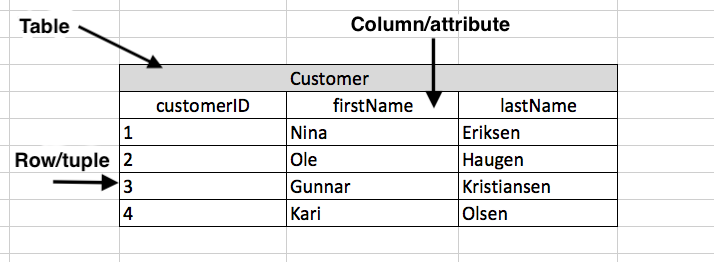
\includegraphics[width=115mm,scale=1]{figures/relational-db-visualised.png}
    \caption{Table named "Customer" containing three attributes and four tuples}
    \label{fig:relational-db-visualised}
\end{figure}

SQL offers a data definition language(DDL) \cite{sql-components}.
The DDL defines the database schema - that is the structure, meaning which attributes the tables consists of, and which tables the database consists of.
It is impossible to add data to the database until a schema has been defined.
The DDL also describes any relational integrities the tables of the database, or the columns of table, may have \cite{sql-constraints}.
In figure \ref{fig:relational-db-relation} a given customer may have several orders but a given order may have one and only one customer associated with it; this is an example of a one-to-many relationship.
In addition to a one-to-many relationship an attribute or table may also have a one-to-one or a many-to-many relationship \cite{sql-relationships}.
Lastly the DDL also defines any security constraints the database may have - such as which users have permissions to read, update or delete the contents of a given table \cite{sql-ddl}.

\begin{figure}
    \centering
    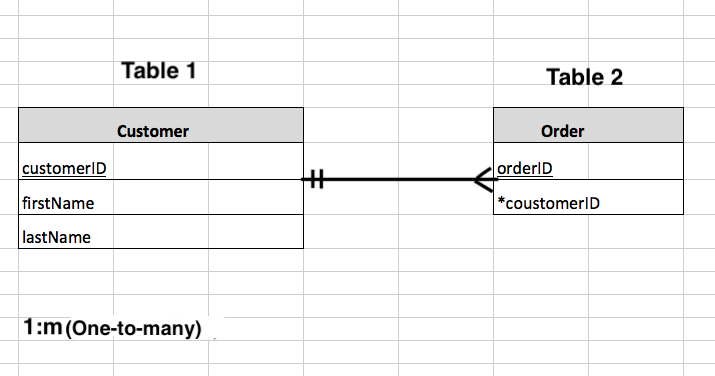
\includegraphics[width=115mm,scale=1]{figures/relational-db-relation.png}
    \caption{One-to-many relation between "Customer" and "Order"}
    \label{fig:relational-db-relation}
\end{figure}

SQL also offers a data manipulation language(DML) \cite{sql-components}.
The DML allows for the insertion of, retrieval of, update of, and deletion of data \cite{sql-dml-options}.
Whenever a tuple is added, updated or removed the tuple must conform to the restraints set by the DDL.
The attempted action will be aborted should there be discrepancies between the constraint of the table or column and the data.
This ensures that the data in the table is accurate and reliable \cite{sql-constraints}.

In addition SQL:
\begin{itemize}
    \item Provides an organized structure as data is defined once, and items referencing the data does so using foreign keys \cite{upwork-sql-adv}.
    \item Reduces data redundancy due to the organized structure \cite{upwork-sql-adv}.
    \item Allows JOIN operations \cite{upwork-sql-adv}.
    The operation allows two or more tables to be combined based on some shared attribute between them.
    The JOIN operation provides the ability to fetch specific data across tables that otherwise would prove cumbersome \cite{sql-joins}.
    \item Provides support for transactions.
    Transactions are essential in databases which require reliable data as they provide a framework for an all-or-nothing approach.
    This means the sequence of involved operations have to succeed in its entirety.
    The database will perform a rollback and raise an error should one of the operations fail \cite{sql-transactions}.
\end{itemize}

\subsection{NoSQL}
A NoSQL(Not only SQL) database provides data storage and data retrieval capabilities that is not modeled using a conventional RDBMS \cite{nosql-not-rdbms}.
Schema-less models are used instead of the traditional RDBMSs.
The most popular models include:
\begin{itemize}
    \item Key-value stores.
    Every item in the database is stored as an attribute name with a corresponding value \cite{mongodb-explains-nosql}.
    The key and value can be anything, and the key acts as a unique identifier for the value \cite{nosql-key-value}.
    \item Document databases.
    Document databases are an extension to key-value stores.
    Documents are structures which can contain many different key-pairs, and documents can even contain other documents.
    The documents can store data in different format, such as XML or JSON.
    Document databases are intended to store semi-sorted data \cite{nosql-document-sort}.
    \item Wide-column stores.
    The data in the database is stored in columns rather than the typical SQL rows.
    A given row can therefore have columns that other rows does not have.
    A wide-column store can be considered a two-dimensional key-value store \cite{infoworld-sql-vs-nosql}.
    \item Graph stores.
    The data in the database is represented as a graph.
    Their intended use is to traverse and navigate relationships.
    These databases use nodes to represent items in the database, and an edge between two nodes represents a relationship between the two items \cite{nosql-graph}.
\end{itemize}

NoSQL is advantageous because it:
\begin{itemize}
    \item Allows for semi-structured or unstructured data in the database.
    This flexible design allows the database to handle changes in structure more easily, and also allows the database to scale with ease \cite{mongodb-adv-nosql}.
    \item Allows for data to be inserted without a schema \cite{omkarsoft-adv-nosql}.
    This is beneficial should data be expected to change during the development of the project.
    \item Scales horizontally rather than vertically \cite{mongodb-adv-nosql}.
    Scaling horizontally allows partitions of data to be scatted across several pieces of hardware in order to store the data in the database.
    By contrast, scaling vertically means replacing already-existing hardware with more powerful hardware \cite{technopedia-nosql-scale}.
\end{itemize}

\subsection{Why SQL is the selected database system}
The assignment provider believes a SQL database system is more suited for the project than that of a NoSQL database system.
The equipment provided at MakerSpace is limited in quantity - as such the data to be stored in the database is also small in scale.
Due to the limited data the schema is simple to define, and as the requirements for the project are unlikely to change at a structural level the flexibility a NoSQL schema provides is not necessary.
The database is also likely to be stored in a limited number of locations and as such the distributed scaling capabilities a NoSQL database system offers is not particularly beneficial.
Overall the benefits provided by a NoSQL database system are not well suited for the project nor the scope of it which makes the SQL database system the preferable choice due to its organized structure, its relational properties and its support for JOIN operations.

\subsection{MariaDB as software}
MariaDB is the assignment providers database management system of choice.
MariaDB is one of the most popular\cite{mariadb-foundation-about} open source relational database management systems in the world \cite{mariadb-about}.
It is a fork of the also popular relational database management system MySQL\cite{mysql-about}.
MariaDB is made by the original developers behind MySQL \cite{mariadb-foundation-about} and it has a large list of sponsors providing financial support including Microsoft and IBM \cite{mariadb-sponsors}.
MariaDB is based on the SQL database system \cite{mariadb-about-searchdatamanagement}.

MariaDB has several notable features.
It is able to handle small and large data alike making it highly scalable, and it allows for rapid access to the data.
MariaDB releases stable releases, and each new release brings speed and stability improvements in addition to new features.
Additionally it places a high value of security - all data is encrypted by default and whenever critical security issues arise a new release is prepared \cite{mariadb-about}.
Lastly MariaDB offers a Node.js connector allowing applications developed on Node.js to connect to MariaDB \cite{mariadb-node-connector}.

\todo{Ikkje bruk several - ver konkret.}
\section{Frontend technology selection} 
The assignment provider wanted a full JavaScript technology stack and as such there were several technologies that could have been chosen for the frontend development.
There are several JavaScript frontend frameworks and libraries freely available and as such this was not a limitation.

The assignment provider ended up choosing Vue.js because of three major factors; the size of the framework, live updating in the browser and the low learning curve it has. Vue.js is comparably smaller than many of the other big JavaScript frameworks. It is roughly 58.8 kB in size. Since the framework is so small it will help with the loading speed of the web application \cite{vue-size}. 

The second major point for choosing Vue.js was the reactivity of Vue. With the reactivity of Vue.js you could update individual components based off of which data had been updated in the database. In Vue.js each component has getters and setters that enables Vue to track each component for when it's been accessed or modified. Each component also has a watcher instance that will be notified when that components setter is triggered. When this happens the watcher will notify Vue to run the component render function on that component again. With this feature there will be no need to update the whole site to show an update in the database \cite{vue-reactivity}. 

\begin{figure}
    \centering
    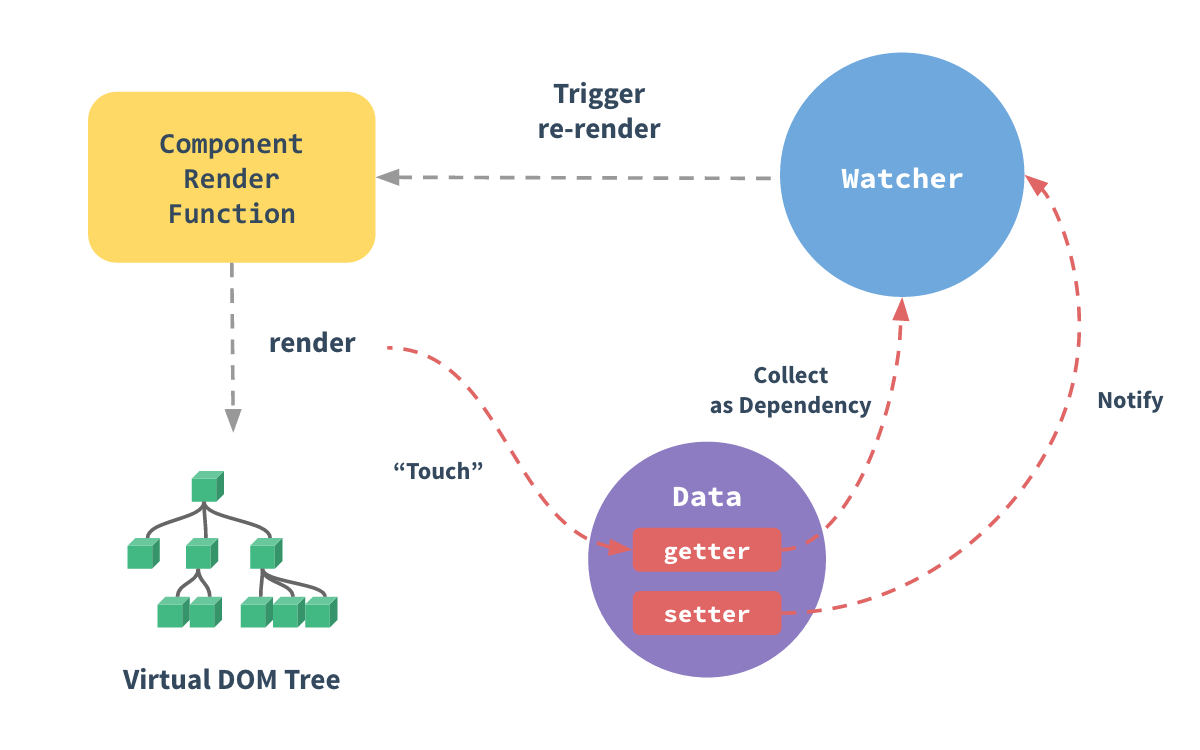
\includegraphics[width=115mm,scale=1]{figures/reactivity.png}
    \caption{Reactivity in Vue.js}
    \label{fig:vue_reactivity}
\end{figure}

The last major point for the group was the low learning curve of Vue.js. With this learning curve it means that the easier parts of Vue.js is easier to learn, but the more complicated components can be harder. This is perfect for the groups project since all the group members are new to Vue.js and can get faster into the programming.

\subsection{Css/Scss}

\section{Backend technology selection}
\todo{en måte: alternativ valg +/- valget}
For the backend technology there are several technologies that could be used. The group had discussed what backend technology to use, and asked the assignment provider to choose. A full JavaScript technology stack was chosen and some of the major backend technologies have been ruled out. Such as Pythons Django, PHP or Javas Spring backend framework. 

JavaScript will be used for the backend, Node.js will be used as the server to create and handle the backend operations needed in the application. Node.js is a JavaScript run-time environment that can run JavaScript code outside of the browser using the V8 JavaScript engine. Node.js runs on a single thread and is able to do this because of the Event Loop. When a request gets sent to Node from the application it will be added to the event queue before being picked up by the Event Loop. The Event Loop will take these requests and send them to the system that Node runs on. Here each request will be sent to different threads and be completed. When the task in done a callback function in the request is activated and the feedback is sent directly back to the application. The reason this event loop is so efficient at handling requests is because it runs asynchronous. So when it receives a request and sends off a callback function for that request. It doesn't need to wait for that callback function to return something before it handles a new request \cite{Node-event-loop}.

\begin{figure}
    \centering
    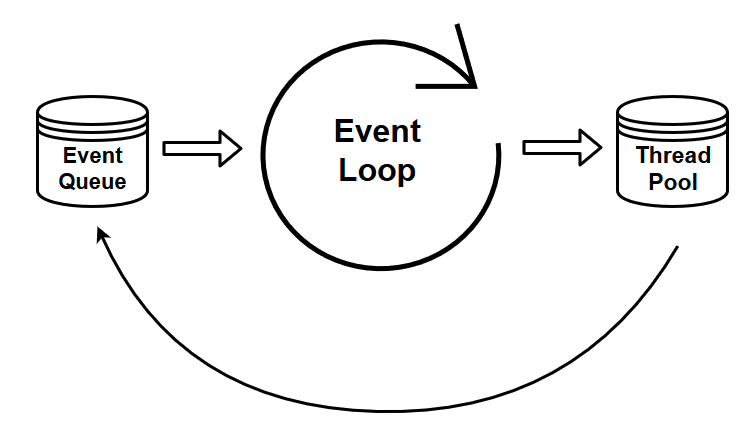
\includegraphics[width=115mm,scale=1]{figures/event_loop.png}
    \caption{Event loop in Node.js}
    \label{fig:Node_Event_Loop}
\end{figure}

\section{Connecting the frontend and the backend}
The frontend needs to be able to connect to the backend to create, read, update or delete resources.
The connection protocol selected is HTTP(Hypertext Transfer Protocol) and HTTPS(Hypertext Transfer Protocol Secure).

\subsection{HTTP and HTTPS}
HTTP is a protocol designed for communication between distributed systems \cite{mozilla_what_is_http}.
The flow of the protocol looks like this \cite{mozilla_http_flow}:
\begin{enumerate}
    \item The client sends an HTTP request to the target host.
    \item The host receives the HTTP request.
    \item The host processes the HTTP request.
    \item The host sends an HTTP response to the client.
    \item The client receives the HTTP response.
\end{enumerate}

HTTPS is an extension of HTTP.
HTTP transmits data in plain text, and as such the protocol is considered insecure as anyone listening or intercepting the traffic can read the data transmitted \cite{http_vs_https}.
HTTPS on the other hand encrypts the data before transmitting it to an external host \cite{https_explained}.
This ensures anyone listening or intercepting the traffic is unable to read the data.
All data can thus pass freely and securely between the two hosts communicating with one another \cite{http_vs_https}.

HTTP/HTTPS lays the foundation for any data exchange \cite{mozilla_http_overview} on the modern web \cite{tutsplus_what_is_http} which makes the protocols the ideal protocols for communication between the frontend and the backend for the project.

\subsection{HTTP status codes}

\subsection{JSON}

\section{Git and GitHub}